\documentclass[10pt,twoside,openright]{memoir}
\usepackage[paperwidth=4.25in, paperheight=6.875in,bindingoffset=.75in]{geometry}
\usepackage[utf8]{inputenc} % If utf8 encoding                                  
\usepackage[T1]{fontenc}    %                                                   
\usepackage[english]{babel} % English please                                    
\usepackage[final]{microtype} % Less badboxes 
\usepackage{tgpagella}
\usepackage{caption}
\usepackage{graphicx}
\usepackage{rotating}

\makeevenhead{headings}%
    {\thepage}{}{}
\makeoddhead{headings}%
    {}{}{\thepage}

\makeatletter
\def\maketitle{%
  \null
  \thispagestyle{empty}%
  \vfill
  \begin{center}\leavevmode
    \normalfont
    {\LARGE\raggedleft \@author\par}%
    \hrulefill\par
    {\huge\raggedright \@title\par}%
    \vskip 1cm
%    {\Large \@date\par}%
  \end{center}%
  \vfill
  \null
  \cleardoublepage
  }
\makeatother

\author{Tao Lin}
\author{Tao Lin}
\title{North American Hamsters}
\date{}










%%% BEGIN DOCUMENT

\begin{document}

\OnehalfSpacing


\let\cleardoublepage\clearpage


\maketitle






\frontmatter


\null\vfill

\begin{flushleft}
\scriptsize
{\em North American Hamsters} is a work of fiction shamelessly stolen from the
internet and reproduced without the author's permission. Names, characters,
places, drugs, MacBooks, grins, and incidents are the product of the author's
imagination or are used fictitiously. Any resemblance to actual persons, 
living or dead (or neither), events, or locales is entirely coincidental. 

\bigskip

Copyright \textcopyright\ 2014 by Tao Lin
\bigskip

Hashtag \#taolin.
\bigskip

All rights reserved. 
\bigskip

Printed in the United States of America by Tony Fader at OfficeMax, a humble
mom-n-pop business located on Capitol Hill in Seattle. 


\end{flushleft}
\let\cleardoublepage\clearpage

\mainmatter
\sloppy

\renewcommand\cftchapteraftersnumb{\normalfont\tiny}
\tableofcontents*




\chapter*{Preface to the 2014 Edition}
\addcontentsline{toc}{chapter}{Preface to the 2014 Edition}
Wow, happy birthday, Allison. Did you know that Tao Lin wrote a series of 
short articles about hamsters, and included hamster illustrations? You're such a
big fan that you probably already knew that. Since you're a big fan, here's a
little booklet of Tao Lin's hamsters. I'd like to think that he wouldn't be 
upset with me for printing this.

\vspace{2em}
\hspace{7em} {\em Tony Fader} 

\hspace{7em} {\em Seattle}

\chapter*{``Non-Eccentric Piano Prodigy'' Hamster}
\addcontentsline{toc}{chapter}{``Non-Eccentric Piano Prodigy'' Hamster}

Despite being considerably ``less rare'' than the {\em ``Eccentric Piano
Prodigy'' Hamster} (due to a much higher reproduction rate and a more balanced
male-to-female ratio, with there however still being more males than females),
not much is known about the {\em ``Non-Eccentric Piano Prodigy'' Hamster} due to
a near-extreme lack of media coverage and an overall, near-complete lack of
public interest (in terms of the hamster itself; its ``wonderful, crisp, and
tender''---according to {\em L Magazine}---recordings actually enjoy very
strong sales in a consistent, recession-proof manner). 
\begin{figure}[t!]
\begin{center}

\includegraphics[width=0.9\textwidth]{img/noneccentricpianoprodigy}
\end{center}
\caption*{{\em ``Non-Eccentric Piano Prodigy'' Hamster}.}
\end{figure}
In a 2013 feature article
in {\em The New York Times Magazine} a {\em ``Non-Eccentric Piano Prodigy'' 
Hamster} named John Thomason atypically received extensive coverage---to the 
extent of 5839 words, of which 4794 were, however, focused on the question of 
``exactly
why'' the article's author has ``long harbored the strong
suspicion'' that the specific {\em ``Non-Eccentric Piano Prodigy'' Hamster}
named John Thomason is ``being non-eccentric on-purpose?'' and therefore,
from a certain ``second level'' perspective, actually way more eccentric
than the {\em ``Eccentric Piano Prodigy'' Hamster}, whose eccentricity is
conveyed ``directly, genetically, honestly, and without
irony---without,'' according to the article's author, Janice Mikaela,
``the questionably legitimate post/meta-artfulness that John Thomason has
subtly deployed in his life and work ever since, as far as my research shows, he
was born.'' The feature article included two full-page photographs
and---interspersed throughout---eight smaller photographs (these smaller
ones focused on her eyes, hands, forearms, mouth, forehead, and hair) of Janice
Mikaela, who was previously known primarily for her eccentric behavior at panel
discussions and ``elegantly outrageous'' ({\em Vogue}) hairstyle, instead of
portraits of the pianist, who also was not interviewed or contacted for the
article.

\vspace{2em}

\noindent
\textbf{Hunting Tips:} Approach the {\em ``Non-Eccentric Piano Prodigy''
Hamster} after a concert asking for its autograph---stunning it, as no one 
cares enough to want its autograph. Ask another question---any question---to 
further destabilize the {\em ``Non-Eccentric Piano Prodigy'' Hamster}'s 
perception of reality (that no one is interested in it) in order to cause 
cardiac arrest, effectively ending its life. Finally, at your leisure, place 
it in a plastic baggie. \\

\newpage

\noindent
\textbf{Cooking Tips:} Baste in a paste of olive oil, wakame, hijiki, tamari 
at a low heat, ``moving it around'' occasionally. Serve over a thick---but not
 too thick---bed of lettuce. Great with red wine, diluted carrot juice,
 or---surprisingly---almond milk.


\begin{sidewaystable}
\begin{center}
  \small
  \begin{tabular}{rl}
  \textbf{Average weight/height (record)} & .9 lbs/3.3" (1.6 lbs/3.9") \\
  \textbf{Average life expectancy (record)} & 18.4 years (36.9 years) \\
  \textbf{Favorite book(s)} & {\em The Mind of God} \\
  \textbf{Favorite band(s)} & anything by Chopin, Brahms \\
  \textbf{Favorite movie(s)} & {\em Eternal Sunshine}  \\
  \textbf{Favorite sexual position} & missionary \\
  \end{tabular}
\end{center}
\caption*{{\em``Non-Eccentric Piano Prodigy'' Hamster} facts.}
\end{sidewaystable}

\chapter*{Factory-Farmed Hamster}
\addcontentsline{toc}{chapter}{Factory-Farmed Hamster}
Force-fed intravenously for the last four days of its eighteen-day,
regimentally/existentially genocidal lives of ``allegory-like'' ``extreme,
sustained, increasing pain,'' the {\em Factory-Farmed Hamster} is by-far the
most common hamster in North America, with a population expected to exceed 200
billion by 2020, a number expected, henceforth, to grow at a rate of 26.4\% per
year, as fast-food companies expand to third-world countries. Born in darkness
in a space not large enough for it to turn around without doing a kind of
back-flip, the {\em Factory-Farmed Hamster} lives its next three days/nights in
a mostly-unconscious haze of bone-level inflammation and intermittent paralysis,
sometimes reflexively jerking forward/backward .5 to .8 inches to prevent its
lower body from ``crystallizing'' in an advanced form of atrophy, while being
force-fed every four hours a mixture of non-organic corn, metastasized
fecal-matter, industrial-strength antibiotics, 4 to 9 varieties of growth
hormones. The next eleven days the {\em Factory-Farmed Hamster} is force-fed
pellets containing the meat/bones/tumors/fur of ``fellow, deceased'' {\em
Factory-Farmed Hamsters} grinded---along with their ``waste,'' which often is
scientifically ``not discernable'' from their ``bodies''---into paste-like
matter that is ``marinated'' 4-8 hours in an antibiotic-hormone mixture and then
dehydrated in gigantic microwaves. 
\begin{figure}[t!]
\begin{center}
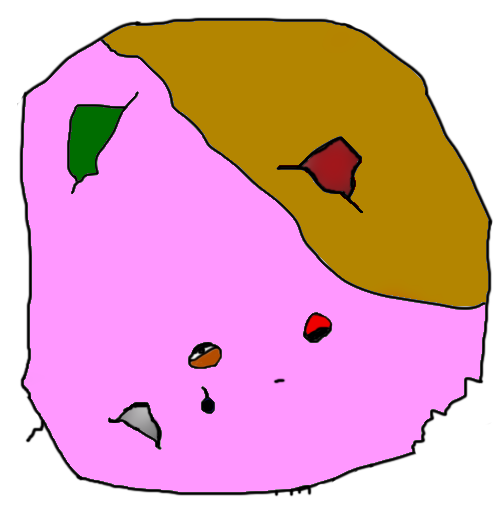
\includegraphics[width=0.9\textwidth]{img/factoryfarmed}
\end{center}
\caption*{{\em Factory-Farmed Hamster}.}
\end{figure}
For the final four days of its ``surreally
bleak existence'' ({\em Mother Jones}) the {\em Factory-Farmed Hamster} is moved
into a larger pen and positioned, within rubber canopies, in a manner allowing
its mouth, facing ``upwards,'' to be uncomplicatedly filled, five times a
day, in a kind of ``funneling action,'' in which former migrant farmhands
without passports, in a job with a 37\% long-term survival rate (many ``succumb''
to various cancers after four years), ``funnel'' (a misnomer, as actually a
``tube'' is used) a non-dehydrated form of ``meat/corn paste'' directly into the
stomach of the {\em Factory-Farmed Hamster}, 73\% of which are, scientifically,
``in comas'' by the morning of the fourth day. In 2010 the FDA declared it
governmentally acceptable for meat labeled ``grade-A'' to continue to be
force-fed up to 35 hours after its source is ``no longer conscious,'' increasing
profits by 18\%. In America an emerging, popular conspiracy theory is that
factory-farmed meat is harmful to those who eat it; connected to or ``in support
of'' that conspiracy, some say, is the taboo, or ``feeling of
shame/inauthenticity/[something],'' of buying organic food, which itself is
related, some say, to the vaguely embarrassing, or ``offensive,'' even, choice
to spend more money on [anything] than ``the lowest amount possible''---a
feeling caused, perhaps, to some degree, by vague intuitions of ```taking part'
in `the conspiracy,' '' along with the influence of the powerful abstraction
most people ultimately convey in the form of the word ``bourgeoisie,'' according
to one conspiracy theorist whose YouTube videos were deleted by YouTube after
pressure from the FDA, who acted ``in preemption,'' according to a fourth-party
conspiracy theorist (whose YouTube videos were also deleted but have since
reappeared on Vimeo), to pressure from the meat/dairy industry.

\noindent
\textbf{Hunting Tips:} Wearing a military-grade gas mask and a
full-body-coverage suit made of space-grade polymers (to protect against deadly
skin lesions and tumors, which have been known to ``fly off'' {\em
Factory-Farmed Hamsters}, when hit by metal doors or simply when they
``burst''), cut a small hole in the corner of a factory-farm shed at night.
Place the {\em Factory-Farmed Hamster} in a garbage bag or shoebox, as it will
not fit in a plastic baggie, taking care not to collapse from empathy-induced
``intense depression'' or ``fear of `evil' in the world,'' as the {\em
Factory-Farmed Hamster} will likely appear ``horrifyingly grotesque'' (Stephen
King via {\em Esquire}), be blind, likely ``crying.''

\vspace{2em}
\noindent
\textbf{Cooking Tips:} Sprinkling antibiotics continuously, grind in entirety
after soaking in a bowl of hydrogen peroxide for 5 to 8 hours. Boil with garlic,
dehydrate, condense into pellets for fish food or ``little balls'' for dog or
cat food. Add [anything] for bulk, grind with antibiotics, and resell to
international or outsourced factory farms as ``grade-A factory farm feed,'' to
second/third-world countries as ``meal packets,'' or fourth-party dog food
producers as ``all-natural, high-grade dog food guaranteed to give your
pet's fur a healthy sheen.''

\begin{sidewaystable}
\begin{center}
  \small
  \begin{tabular}{rl}
  \textbf{Average weight/height (record)} & 4.4 lbs/4.2" (4.8 lbs/4.6") \\
  \textbf{Average life expectancy (record)} & .049 years (.049 years) \\
  \textbf{Favorite book(s)} & doesn't know what a ``book'' is \\
  \textbf{Favorite band(s)} & doesn't know what a ``band'' is \\
  \textbf{Favorite movie(s)} & doesn't know what a ``movie'' is \\
  \textbf{Favorite sexual position} & doesn't know what ``sex'' is \\
  \end{tabular}
\end{center}
\caption*{{\em Factory-Farmed Hamster} facts.}
\end{sidewaystable}


\end{document}

